\documentclass{article}
\usepackage{microtype}
\usepackage{graphicx}
\usepackage{subcaption}
\usepackage{booktabs}
\usepackage{hyperref}
\usepackage{icml2026}
\usepackage{amsmath,amssymb,amsthm,mathtools}
\usepackage{enumitem}
\newtheorem{theorem}{Theorem}
\newtheorem{proposition}{Proposition}
\newcommand{\E}{\mathbb E}
\newcommand{\R}{\mathbb R}
\newcommand{\one}{\mathbf 1}
\newcommand{\gate}{\tau_\star}
\newcommand{\given}{\,\vert\,}
\newcommand{\RLLow}{0.351}
\newcommand{\SLLow}{0.005}
\newcommand{\RCLow}{0.210}
\newcommand{\SCLow}{0.008}
\newcommand{\RLMid}{0.477}
\newcommand{\SLMid}{0.007}
\newcommand{\RCMid}{1.963}
\newcommand{\SCMid}{0.074}
\newcommand{\RLHigh}{0.577}
\newcommand{\SLHigh}{0.013}
\newcommand{\RCHigh}{16.519}
\newcommand{\SCHigh}{0.641}
\newcommand{\FBc}{0.085}
\newcommand{\FBcse}{0.003}
\newcommand{\SBMc}{1.441}
\newcommand{\SBMcse}{0.056}
\newcommand{\SBMcc}{0.057}
\newcommand{\SBMccse}{0.002}
\newcommand{\FBl}{0.333}
\newcommand{\FBlse}{0.010}
\newcommand{\FBcl}{0.059}
\newcommand{\FBclse}{0.002}
\newcommand{\Reglcluster}{0.582}
\newcommand{\Reglclusterse}{0.016}
\newcommand{\CVLow}{0.256}
\newcommand{\CVLowse}{0.011}
\newcommand{\ChooseCLow}{65.3}
\newcommand{\CVMid}{1.312}
\newcommand{\CVMidse}{0.114}
\newcommand{\ChooseCMid}{28.0}
\newcommand{\CVHigh}{10.299}
\newcommand{\CVHighse}{1.342}
\newcommand{\ChooseCHigh}{23.3}
\newcommand{\QuadBiasLow}{-1.173}
\newcommand{\QuadBiasLowse}{0.010}
\newcommand{\QuadBiasMid}{0.004}
\newcommand{\QuadBiasMidse}{0.007}
\newcommand{\QuadBiasHigh}{1.161}
\newcommand{\QuadBiasHighse}{0.009}
\newcommand{\CoverIIDB}{35.5}
\newcommand{\CoverOracleB}{97.2}
\newcommand{\CoverIIDC}{12.0}
\newcommand{\CoverOracleC}{95.0}
\newcommand{\SharpLow}{1.369}
\newcommand{\LooseLow}{5.755}
\newcommand{\SharpMid}{2.170}
\newcommand{\LooseMid}{13.091}
\newcommand{\SharpHigh}{2.596}
\newcommand{\LooseHigh}{27.958}
\newcommand{\ThresholdHighValid}{0}
\newcommand{\ThresholdMidValid}{31.8}
\newcommand{\ThresholdUB}{1.55e-09}
\newcommand{\TrimAll}{0.085}
\newcommand{\TrimAllse}{0.003}
\newcommand{\KeptAll}{4039}
\newcommand{\RandomAll}{0.085}
\newcommand{\RandomAllse}{0.003}
\newcommand{\TrimTwenty}{1.806}
\newcommand{\TrimTwentyse}{0.067}
\newcommand{\KeptTwenty}{2341}
\newcommand{\RandomTwenty}{0.119}
\newcommand{\RandomTwentyse}{0.005}
\newcommand{\TrimHundred}{58.034}
\newcommand{\TrimHundredse}{3.398}
\newcommand{\KeptHundred}{491}
\newcommand{\RandomHundred}{0.270}
\newcommand{\RandomHundredse}{0.010}
\newcommand{\BaseAssignments}{12000}
\newcommand{\IdentityMaxZ}{4.045}

\icmltitlerunning{Endpoint Geometry for Regression GATE Estimation}
\begin{document}
\raggedbottom
\twocolumn[
\icmltitle{Endpoint Geometry for Regression GATE Estimation:\\
Sharp Curvature Bounds and Network Stress Tests}
\begin{icmlauthorlist}
\icmlauthor{Anonymous Authors}{anon}
\end{icmlauthorlist}
\icmlaffiliation{anon}{Anonymous Institution}
\icmlkeywords{network interference, global treatment effects, regression, sensitivity analysis}
\vskip 0.3in
]
\printAffiliationsAndNotice{}
\begin{abstract}
Regression can estimate the global average treatment effect (GATE) under interference by predicting all-treated and all-control outcomes, but those endpoints can be far from the experimental exposures.
We express its conditional error through endpoint weights and derive a sharp, computable worst-case bias bound under a common exposure-response curvature constraint.
Complement symmetry explains an exact zero-average-bias exception for quadratic interference, while a coupling argument demonstrates failure when high-exposure responses are almost never observed.
On fixed synthetic networks and the public ego-Facebook graph, repeated CPU simulations show that correctly specifying a cubic response can greatly increase GATE error: on degree-128 regular graphs its RMSE is \RCHigh{}, versus \RLHigh{} for a misspecified linear fit.
Prediction-based selection, clustering, and correlated noise produce distinct tradeoffs; low-degree observation ablations reveal why mean degree alone is inadequate.
The resulting sensitivity intervals are valid under stated curvature and noise assumptions but can be wide; neither ordinary predictive accuracy nor model correctness alone certifies accurate GATE estimation.
\end{abstract}

\section{Introduction}
In an A/B test with social or marketplace interactions, one unit's treatment can affect another's outcome. The platform may care about replacing the entire system, so its target is the difference between everyone treated and everyone controlled, rather than the direct effect at the experiment's treatment saturation. A regression that uses own treatment and neighbors' treatment can predict both counterfactual regimes \citep{chin2019}. The central difficulty is that an individually randomized experiment may contain little information about either regime.

This paper studies \emph{how accurate these endpoint predictions can be}, distinguishing noise amplification from response misspecification. These are different obstacles. Adding a correct nonlinear feature can remove bias while amplifying noise. Changing the randomization can expand exposure support while changing the alignment of treatment, exposure, and correlated shocks. Even the statement ``nonlinearity causes bias'' has exceptions: complement symmetry makes a linear regression average-unbiased for a quadratic GATE at half saturation.

Our contribution is a focused diagnostic analysis, not a new regression-adjustment algorithm. First, we specialize the Peano-kernel representation of linear approximation error to the network GATE contrast. This produces a sharp finite-sample curvature sensitivity bound and an honest conditional Gaussian interval when curvature and noise covariance are supplied. Second, we pair this result with an exact symmetry argument and a finite-experiment indistinguishability bound, separating a benign misspecification from an unobserved-threshold failure. Third, controlled simulations test these distinctions on several topologies, designs, response laws, and noise structures. A public-graph ablation and a prediction-selection experiment examine mechanisms behind the observed rankings.

The scope is deliberately limited. The sharp bound assumes a common scalar neighbor-exposure response, and the experiments use synthetic continuous outcomes on known fixed graphs. Covariance-based intervals below use known simulation covariance, isolating extrapolation from covariance estimation. We report Monte Carlo uncertainty and failures of estimability; we do not claim uniformly optimal regression or inference under unrestricted interference.

\section{Related Work}
\citet{aronow2017} formulate interference using an exposure mapping and design-based inverse-probability estimation. This clarifies that an estimator's validity depends on which assignments share potential outcomes. \citet{ugander2013} use graph cluster randomization to change exposure probabilities, including full-neighborhood exposure; their analysis already identifies large variance as a concern. \citet{eckles2017} study bias reduction through both design and the inclusion of neighbors' assignments in analysis. These establish the importance of studying design and analysis jointly.

\citet{chin2019} explicitly estimate GATE by regression prediction under global treatment and control, characterize a linear-model setting, and propose flexible regression and resampling inference. \citet{han2023} generate and select graph/treatment features and develop block-bootstrap inference. We use small fixed dictionaries to isolate endpoint information rather than replicate their feature-selection algorithms. We make no claim that regression adjustment, exposure features, or clustering are novel. Our specific addition is a sharp curvature sensitivity functional for endpoint-calibrated weights, alongside complementary success/failure calculations and stress tests. Literature consultation was intentionally confined to the supplied starter papers; a comprehensive priority claim is unwarranted.

\section{Setup and Estimators}
Let $A$ be a known undirected loop-free adjacency matrix, $d_i>0$, and $P=D^{-1}A$. For binary assignment $z\in\{0,1\}^n$, define one-hop exposure $s=Pz$ and two-step walk exposure $t=P^2z$. The latter includes return walks. Write
\begin{equation}
Y_i(z)=\mu_i(z)+\varepsilon_i,\qquad
\gate=\frac1n\sum_i\{\mu_i(\one)-\mu_i(0)\}.
\label{eq:target}
\end{equation}
The mean-zero noise vector is independent of assignment, with covariance $\Sigma$. A draw of $\varepsilon$ can be shared across all potential outcomes within a repetition, so it cancels from the finite-population global contrast as well. Repetitions redraw assignment and noise, conditional on a fixed graph and covariate.

Given feature matrix $X=X(z)$ and endpoint contrast
\begin{equation}
c=\frac1n\sum_i\{\phi_i(\one)-\phi_i(0)\},
\end{equation}
the OLS plug-in estimator is $\widehat\tau=c^\top X^+Y=a^\top Y$. Here $X^+$ is the Moore--Penrose inverse. The contrast must be estimable, $c\in\operatorname{row}(X)$; a numerical prediction from a pseudoinverse does not establish identification. For an estimable contrast, $a=X(X^\top X)^+c$ and $X^\top a=c$.

All regressions include an intercept and fixed pretreatment covariate $x$. OLS-L adds $(z,s)$; OLS-Q adds $(s-1/2)^2$; OLS-C additionally adds $(s-1/2)^3$; OLS-2H instead adds $t$ to OLS-L. Centering is a numerical reparameterization. Endpoint contrasts for these added terms are $0$, $1/4$, and $1$, respectively. Ridge-C standardizes the OLS-C columns and penalizes all slopes with fixed penalty 10; it has no outcome-based tuning. It is a bias--variance comparator, and generally lacks the calibration needed for our curvature theorem.

Baselines are the treated-minus-control mean (DM) and Horvitz--Thompson (HT) under closed-neighborhood full exposure. HT weights equal $\{\one(z_i=s_i=1)-\one(z_i=s_i=0)\}/(n\pi_i)$. At half saturation, $\pi_i=2^{-(d_i+1)}$ under independent assignment and $2^{-q_i}$ under cluster assignment, where $q_i$ counts distinct groups in the closed neighborhood. This HT is unbiased for the four one-hop laws used here, but \emph{not} the two-hop law. Very rare exposures make its empirical RMSE difficult to assess; we report it separately rather than treating absent rare events as evidence of stability.

\section{Endpoint Error and Sensitivity}
\subsection{An exact decomposition}
For any fixed candidate linear estimator whose weights depend on $z$ and the graph, not on outcomes,
\begin{align}
b(z)&=a^\top\mu(z)-\gate,\nonumber\\
\E[(\widehat\tau-\gate)^2\given z]
 &=b(z)^2+a^\top\Sigma a.
\label{eq:mse}
\end{align}
Under a correctly specified feature model with the correct endpoint contrast, $b(z)=0$. Under independent homoskedastic noise, the variance is $\sigma^2\|a\|_2^2$. Thus a model can be correct and still inaccurate because its endpoint weights have a large norm. Ordinary prediction error averages loss near observed exposures; it need not control this contrast. Equation~\eqref{eq:mse} remains an identity under misspecification, but $b(z)$ requires the unobserved response and is not an observable certificate.

\subsection{A sharp curvature bound}
For the following result, impose a common exposure-response model
\begin{equation}
\begin{gathered}
\mu_i(z)=\alpha+\beta x_i+\theta z_i+h(s_i),\\
h\in C^2[0,1],\qquad \|h''\|_\infty\le M.
\end{gathered}
\label{eq:smooth}
\end{equation}
Then $\gate=\theta+h(1)-h(0)$. The constant $M$ is a substantive sensitivity parameter, not something identified from concentrated experimental exposures.

\begin{theorem}[Sharp conditional curvature sensitivity]
\label{thm:peano}
Suppose $a^\top\one=a^\top x=0$ and $a^\top z=a^\top s=1$. Define
\begin{align}
K_a(u)&=\sum_i a_i(s_i-u)_+-(1-u),\nonumber\\
B_M(a,s)&=M\int_0^1|K_a(u)|\,du.
\label{eq:kernel}
\end{align}
Under \eqref{eq:smooth}, $|b(z)|\le B_M(a,s)$. This bound is sharp as a supremum over the stated curvature class for the fixed design and weights. Moreover,
\begin{equation}
B_M(a,s)\le \frac M2\sum_i|a_i|s_i(1-s_i).
\label{eq:triangle}
\end{equation}
If noise is conditionally Gaussian with known $\Sigma$, the interval
\begin{equation}
\widehat\tau\ \pm\ \left\{B_M(a,s)+1.96\sqrt{a^\top\Sigma a}\right\}
\label{eq:ci}
\end{equation}
has conditional coverage at least $95\%$ for every response in the class, up to the rounding of the Gaussian quantile.
\end{theorem}

\emph{Proof sketch.} The functional $Lh=\sum_i a_i h(s_i)-h(1)+h(0)$ annihilates affine functions. Taylor's integral formula gives $Lh=\int K_a h''$. Taking $h''$ arbitrarily close to $M\operatorname{sign}(K_a)$ proves sharpness. Subtracting each observation's endpoint chord and applying the triangle inequality gives \eqref{eq:triangle}. The noise event $|a^\top\varepsilon|\le1.96\sqrt{a^\top\Sigma a}$ implies coverage. Full details are in Appendix~\ref{app:proofs}.

The kernel is piecewise linear with knots at $0,s_1,\ldots,s_n,1$. Its absolute integral is computed exactly by splitting at zero crossings; no numerical optimization is needed. The theorem applies to the fixed OLS dictionaries, including misspecified ones, whenever the endpoint contrast is estimable. It does not apply automatically to outcome-selected models, arbitrary heterogeneous $h_i$, omitted two-hop responses, or noncalibrated ridge weights. If $M$ or $\Sigma$ is unknown, the displayed interval is a sensitivity calculation, not an automatically valid fitted confidence interval.

\begin{figure*}[t]
\centering
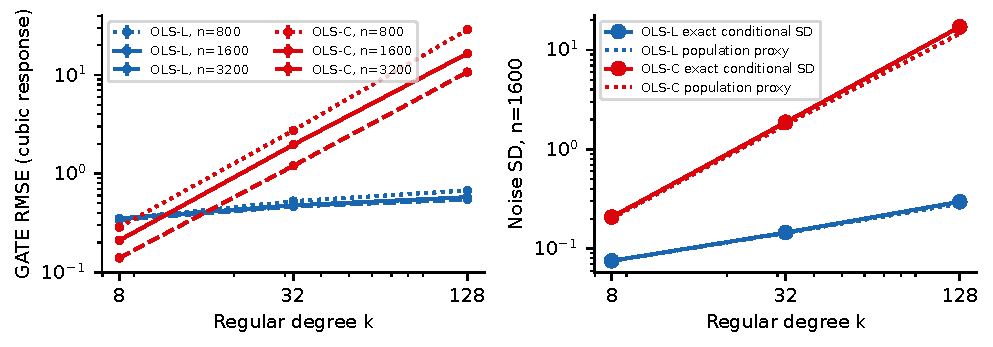
\includegraphics[width=\textwidth]{../figures/degree_scaling.pdf}
\caption{Cubic response under independent half-saturation assignment. Left: GATE RMSE across sample sizes and regular degrees; bars are $\pm1.96$ Monte Carlo SE. Right: root-mean conditional noise variance at $n=1600$, compared with population-information proxies (dotted). Correctly specified OLS-C pays a steep noise penalty. Each point uses 400 repetitions.}
\label{fig:degree}
\end{figure*}

\subsection{Two contrasting misspecifications}
\begin{proposition}[Quadratic cancellation]
\label{prop:symmetry}
Under \eqref{eq:smooth} with $h(s)=\gamma s^2$, OLS-L has zero assignment-average conditional bias for any complement-symmetric assignment distribution, on a complement-invariant set of estimable assignments.
\end{proposition}
Indeed, $a(\one-z)=-a(z)$, so the quadratic bias $\gamma\{a(z)^\top s^2-1\}$ changes sign under complementation. This is average cancellation, not conditional correctness. Both independent and cluster half-saturation designs have this symmetry. Changing the treatment probability breaks it.

The opposite extreme is a response that activates only where the experiment almost never goes. Compare $\mu_i^0=1+\beta x_i+z_i$ and $\mu_i^1=\mu_i^0+\Delta\one(s_i\ge q)$, whose GATEs differ by $\Delta$. Couple their assignments and noise. Their entire observed datasets coincide whenever no exposure exceeds $q$. If this event fails with probability at most $\delta$, every estimator $T$ satisfies
\begin{equation}
\max_{j\in\{0,1\}}\E_j[(T-\tau_j)^2]
\ \ge\ \frac{\Delta^2}{4}(1-\delta).
\label{eq:lower}
\end{equation}
For independent Bernoulli($p$) assignment on a degree-$k$ regular graph,
\begin{equation}
\delta\le \min\{1,n\Pr[\mathrm{Bin}(k,p)\ge\lceil qk\rceil]\}.
\end{equation}
No independence of exposures across nodes is required. The bound concerns a two-response class without knowledge of which response is true. The threshold response is outside the smoothness class of Theorem~\ref{thm:peano}.

\subsection{A population-information benchmark}
For a regular graph at half saturation, a single node has $s\sim\mathrm{Bin}(k,1/2)/k$, independent of its own treatment. Replacing the random Gram matrix by its expectation gives noise-variance proxies
\begin{align}
V_{\rm L}^{\rm pop}&=\frac{\sigma^2}{n}(4+4k),\nonumber\\
V_{\rm C}^{\rm pop}&=\frac{\sigma^2}{n}\left(4+4k+\frac23 k(k-1)(k-2)\right).
\label{eq:proxy}
\end{align}
These follow by orthogonalizing the centered cubic under the binomial distribution (Appendix~\ref{app:proxy}). They highlight $k/n$ versus $k^3/n$ information demands. They are \emph{not} formulas for the expectation of the inverse random Gram matrix, and imply no universal network asymptotic rate. The discrepancy from exact conditional variance in Figure~\ref{fig:degree} is itself relevant at finite $n$.

\section{Experimental Design}
\paragraph{Graphs and randomization.}
We fix six graphs: regular graphs with $n=1600$, $k\in\{8,32,128\}$; a 40-block SBM, 40 nodes per block, within-edge probability $0.6$, between-edge probability $4/1560$; a Barab\'asi--Albert (BA) graph with $n=1600$, attachment parameter 16; and the full SNAP ego-Facebook graph, $4039$ nodes and $88234$ undirected edges \citep{snap}. We use the downloaded edge list unchanged except for sorted relabeling. No real outcomes or user attributes enter the study. Independent assignment treats each node with probability $1/2$. Cluster assignment treats each fixed group independently with that probability; groups are planted SBM blocks or Louvain communities at resolution 2, fixed seed. Appendix~\ref{app:protocol} gives graph statistics and complete implementation details.

\paragraph{Responses and noise.}
Each graph has a fixed standardized synthetic covariate obtained from $\log(1+d_i)$ plus independent standard Gaussian draws. Conditional means are
\begin{equation}
\begin{gathered}
\mu_i=1+0.5x_i+z_i+g_i,\\
g\in\{2s,\ 2s^2,\ 2s^3,\ 2\one(s\ge.8),\ s+t\}.
\end{gathered}
\end{equation}
Every true GATE is exactly 3. Main noise is iid Gaussian with $\sigma=0.5$. A second suite uses $\varepsilon_i=\sigma\{\sqrt{1-\rho}\,\xi_i+\sqrt\rho\,\eta_{G(i)}\}$ with $\rho=1/2$ and independent standard Gaussian node and fixed-group shocks. Correlation groups are the same fixed groups under both assignment designs; assignment does not create noise dependence.

\paragraph{Evaluation.}
We run 400 repetitions per graph/design in each main and correlated-noise suite, using common assignment and noise across methods and response laws. Scaling adds $n=800,3200$ at each regular degree, 400 repetitions each. We measure bias, RMSE, their Monte Carlo SEs, conditional error components, and coverage using true covariance. RMSE measures total error in the platform's target units; bias distinguishes systematic extrapolation error from noisy estimates. Bias MCSE is the error SD divided by $\sqrt R$; RMSE MCSE uses the delta method on squared errors. Figure bars use $1.96$ MCSE, while table parentheses give one MCSE. These quantify repetition uncertainty conditional on each graph, not uncertainty over graph populations.

For cubic responses, a separate experiment uses 150 repetitions per degree, a 70/30 random node split, and held-out noisy-outcome MSE to select among OLS-L/Q/C, followed by full-data refitting. A 60-tree random forest (RF), minimum leaf size 10, is a flexible prediction comparator with the same inputs $(x,z,s)$. Test labels are not used for fitting candidates; treatment/exposure features are computed on the full known graph. This is transductive within-experiment prediction, not independent-network validation. A saturation check varies $p\in\{.2,.5,.8\}$ for quadratic responses. An exploratory Facebook ablation removes low-degree \emph{outcome observations} from the fit while retaining the graph, exposures, and full-population target; it uses 400 paired repetitions and an equal-size random-deletion control. These are exploratory follow-ups to the main results.

\section{Results}
\subsection{Correct specification can increase total error}
On regular graphs with degree 8, cubic-response RMSE falls from $\RLLow{}$ (MCSE $\SLLow{}$) with OLS-L to $\RCLow{}$ ($\SCLow{}$) with correctly specified OLS-C. At degree 32, OLS-C instead has RMSE $\RCMid{}$ ($\SCMid{}$) versus $\RLMid{}$ ($\SLMid{}$); at degree 128 the comparison is $\RCHigh{}$ ($\SCHigh{}$) versus $\RLHigh{}$ ($\SLHigh{}$). Exact conditional noise variance explains this reversal (Figure~\ref{fig:degree}), while OLS-L keeps approximation bias. Increasing $n$ helps both methods in these fixed-degree comparisons but does not eliminate OLS-L's cubic bias.

The correctly specified cubic fit is not uniformly preferable, even with modest regularization (Table~\ref{tab:cubic}). Conversely, the two-hop law requires more than polynomial one-hop terms: OLS-2H removes its conditional bias, but has its own variance cost. Full results for all laws are in Appendix~\ref{app:full}; we report both favorable and unfavorable cases. The exact decomposition is checked against empirical squared error in the supplied summaries, without expecting identical finite-repetition values. An exhaustive small-graph HT check and direct numerical curvature/variance checks also pass.

\begin{table*}[t]
\centering\scriptsize
\caption{Cubic-response GATE RMSE (Monte Carlo SE) over 400 repetitions per row. Bern.: independent Bernoulli assignment. Methods share outcomes within each row; assignment designs use independent draws. Full-exposure HT is reported separately because of unresolved rare-event tails.}
\label{tab:cubic}
\begin{tabular}{llcccccc}
\toprule
Graph & Assignment & DM & OLS-L & OLS-Q & OLS-C & OLS-2H & Ridge-C \\
\midrule
Regular 8 & Bern. & $2.000\,(0.002)$ & $0.351\,(0.005)$ & $0.341\,(0.004)$ & $0.210\,(0.008)$ & $0.398\,(0.010)$ & $0.207\,(0.008)$ \\
Regular 8 & Cluster & $1.483\,(0.005)$ & $0.423\,(0.013)$ & $0.289\,(0.004)$ & $0.137\,(0.005)$ & $0.473\,(0.015)$ & $0.132\,(0.005)$ \\
Regular 32 & Bern. & $2.000\,(0.002)$ & $0.477\,(0.007)$ & $0.478\,(0.007)$ & $1.963\,(0.074)$ & $0.942\,(0.031)$ & $1.911\,(0.072)$ \\
Regular 32 & Cluster & $1.816\,(0.003)$ & $0.582\,(0.016)$ & $0.495\,(0.009)$ & $1.510\,(0.052)$ & $0.966\,(0.034)$ & $1.425\,(0.049)$ \\
Regular 128 & Bern. & $2.001\,(0.002)$ & $0.577\,(0.013)$ & $0.582\,(0.013)$ & $16.519\,(0.641)$ & $3.610\,(0.128)$ & $16.046\,(0.628)$ \\
Regular 128 & Cluster & $1.934\,(0.002)$ & $0.624\,(0.019)$ & $0.718\,(0.027)$ & $15.044\,(0.572)$ & $3.537\,(0.130)$ & $12.443\,(0.466)$ \\
SBM & Bern. & $2.003\,(0.002)$ & $0.467\,(0.007)$ & $0.467\,(0.007)$ & $1.441\,(0.056)$ & $0.511\,(0.011)$ & $1.408\,(0.055)$ \\
SBM & Cluster & $0.410\,(0.004)$ & $0.095\,(0.003)$ & $0.054\,(0.002)$ & $0.057\,(0.002)$ & $0.240\,(0.008)$ & $0.051\,(0.002)$ \\
BA & Bern. & $2.001\,(0.002)$ & $0.471\,(0.008)$ & $0.459\,(0.006)$ & $0.999\,(0.036)$ & $0.902\,(0.031)$ & $0.976\,(0.035)$ \\
BA & Cluster & $1.785\,(0.003)$ & $0.564\,(0.015)$ & $0.466\,(0.008)$ & $0.829\,(0.031)$ & $0.995\,(0.032)$ & $0.788\,(0.029)$ \\
Facebook & Bern. & $2.001\,(0.001)$ & $0.333\,(0.010)$ & $0.235\,(0.003)$ & $0.085\,(0.003)$ & $0.412\,(0.009)$ & $0.085\,(0.003)$ \\
Facebook & Cluster & $0.230\,(0.007)$ & $0.059\,(0.002)$ & $0.028\,(0.001)$ & $0.020\,(0.001)$ & $0.064\,(0.002)$ & $0.020\,(0.001)$ \\
\bottomrule
\end{tabular}
\end{table*}

\begin{figure*}[t]
\centering
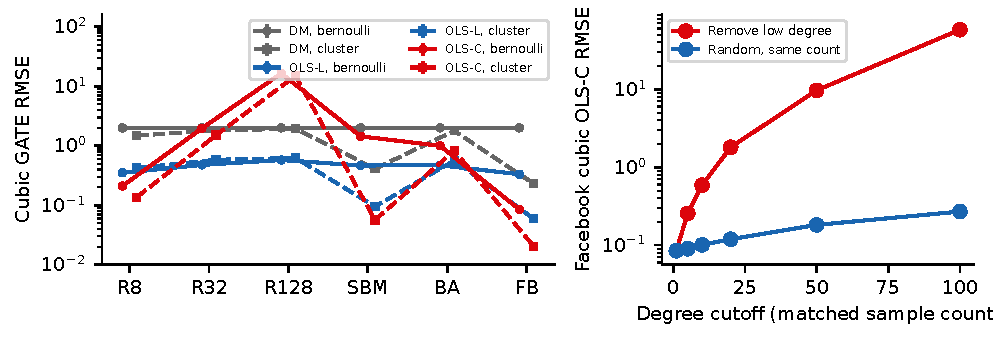
\includegraphics[width=\textwidth]{../figures/design_support.pdf}
\caption{Design and topology affect endpoint information. Left: cubic-response RMSE under independent and cluster assignment, 400 repetitions each. Right: Facebook OLS-C after excluding low-degree outcome observations; the graph and population target are retained. Bars are $\pm1.96$ MCSE. Random deletion retains the same number of outcomes at each cutoff, providing a sample-size control.}
\label{fig:design}
\end{figure*}

\subsection{Network support matters beyond mean degree}
Cluster assignment improves cubic OLS-C on the SBM from $\SBMc{}$ ($\SBMcse{}$) to $\SBMcc{}$ ($\SBMccse{}$), and also improves it on Facebook (Table~\ref{tab:cubic}). These partitions keep many edges inside treatment groups and expand exposures. The effect is not uniform: degree-32 regular OLS-L worsens from $\RLMid{}$ to $\Reglcluster{}$ ($\Reglclusterse{}$), while its OLS-C improves. Complement symmetry preserves quadratic average-unbiasedness even though conditional variance and bias can change.

Facebook's average degree exceeds that of the degree-32 regular graph, yet cubic OLS-C RMSE is only $\FBc{}$ ($\FBcse{}$) under independent assignment. Low-degree nodes provide exposures closer to the endpoints. Removing observations with degree below 20, while keeping all treatment/exposure calculations, retains $\KeptTwenty{}$ nodes and raises RMSE to $\TrimTwenty{}$ ($\TrimTwentyse{}$). A degree-100 cutoff retains $\KeptHundred{}$ and raises it to $\TrimHundred{}$ ($\TrimHundredse{}$). Figure~\ref{fig:design} shows intermediate cutoffs. Random deletion with these same retained sample sizes yields RMSE $\RandomTwenty{}$ ($\RandomTwentyse{}$) and $\RandomHundred{}$ ($\RandomHundredse{}$), respectively. This control supports an exposure-information explanation beyond sample size under the homogeneous cubic law; it does not justify transferring low-degree effects under heterogeneous response laws.

\subsection{Prediction validation does not certify the endpoint}
The held-out MSEs of polynomial candidates nearly coincide at high degree (Figure~\ref{fig:prediction}). At degree 128, the selector chooses cubic regression in $\ChooseCHigh{}\%$ of repetitions, and its GATE RMSE is $\CVHigh{}$ ($\CVHighse{}$). Thus occasional selection of a high-variance endpoint predictor dominates total error. At degree 8, selection has RMSE $\CVLow{}$ ($\CVLowse{}$), between fixed linear and cubic fits in this separate experiment. We do not claim that validation always fails: it distinguishes more at low degree, and it can be appropriate for its prediction objective. RF's endpoint contrast is poor here despite reasonable prediction, consistent with its inability to extrapolate outside observed feature ranges. RF also has worse predictive MSE than polynomial candidates, so this experiment does not establish that its predictive performance is superior.

\begin{figure*}[t]
\centering
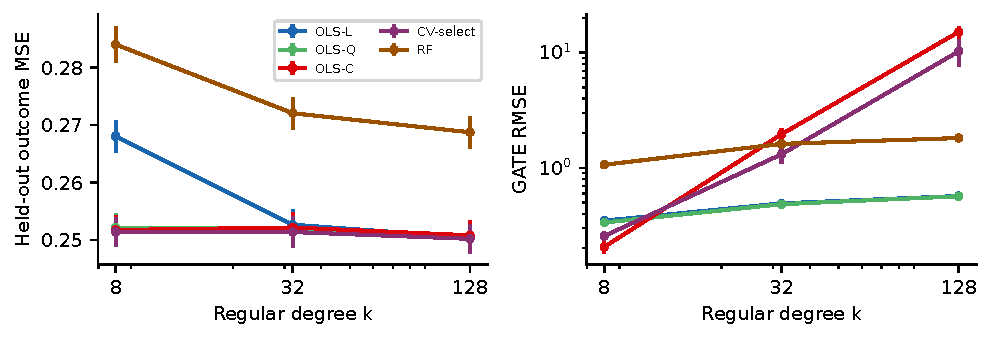
\includegraphics[width=\textwidth]{../figures/prediction.pdf}
\caption{Cubic response, 150 independent validation repetitions per degree. Left: held-out noisy-outcome MSE. The selected validation score is a minimum and is optimistically biased as a risk estimate. Right: full-data GATE RMSE from the same repetitions. Bars are $\pm1.96$ MCSE. The prediction and GATE objectives separate as exposures concentrate.}
\label{fig:prediction}
\end{figure*}

\begin{figure*}[t]
\centering
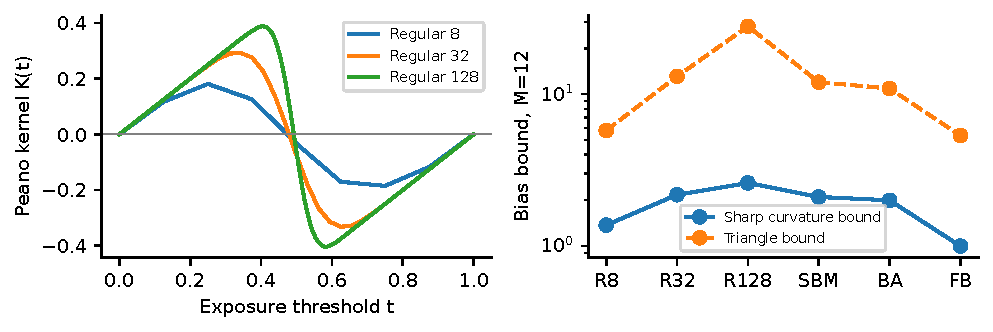
\includegraphics[width=\textwidth]{../figures/sensitivity.pdf}
\caption{Curvature sensitivity of OLS-L. Left: exact Peano kernels for the first independent assignment on each regular graph, illustrating realized weight geometry. Right: mean cubic-curvature bias bounds ($M=12$), 400 repetitions, with $\pm1.96$ MCSE. Sharpness reduces conservatism relative to summing pointwise chord bounds, but it does not supply missing endpoint observations.}
\label{fig:sensitivity}
\end{figure*}

\subsection{Benign cancellation and unsupported thresholds}
The quadratic check supports Proposition~\ref{prop:symmetry}: OLS-L bias at $p=.5$ is $\QuadBiasMid{}$ (MCSE $\QuadBiasMidse{}$). At $p=.2$ and $.8$, it is $\QuadBiasLow{}$ ($\QuadBiasLowse{}$) and $\QuadBiasHigh{}$ ($\QuadBiasHighse{}$), respectively. This is a response/design interaction, not a universal failure of linear regression on nonlinear outcomes. Figure~\ref{fig:extra} shows the comparison with a binomial population projection.

For the degree-128 threshold law, the correctly specified indicator coefficient is inestimable in all 400 repetitions under either design (Appendix~\ref{app:oracle}). Independent-assignment exposure probability has the exact union upper bound \texttt{\ThresholdUB{}}. Equation~\eqref{eq:lower} therefore gives a near-unit minimax MSE lower bound for the two-response class with $\Delta=2$, even with noiseless outcomes. At degree 32, the oracle indicator contrast is estimable in only $\ThresholdMidValid{}\%$ of independent assignments. We report conditional-on-estimability RMSE separately; silently dropping the other assignments would overstate its usefulness. Polynomial fits remain numerically estimable but cannot identify an unseen step without extra assumptions.

\subsection{Sensitivity is valid but can be costly}
The sharp curvature bound is substantially smaller than the triangle bound, yet often remains large (Figure~\ref{fig:sensitivity}). With cubic curvature $M=12$, average sharp bounds for regular degrees 8, 32, and 128 are $\SharpLow{}$, $\SharpMid{}$, and $\SharpHigh{}$; the corresponding triangle bounds are $\LooseLow{}$, $\LooseMid{}$, and $\LooseHigh{}$. Sensitivity coverage is conservative in these runs; coverage and widths are supplied for each graph/design in the result files. High coverage here does not mean high precision. The theorem's sharpness is worst-case over a curvature class, while the cubic law is only one member, so its actual bias can be much smaller.

Noise dependence is a separate limitation. In the correlated-noise linear law, iid-covariance intervals on Facebook cover only $\CoverIIDB{}\%$ under independent assignment and $\CoverIIDC{}\%$ under cluster assignment. Using true covariance restores $\CoverOracleB{}\%$ and $\CoverOracleC{}\%$, respectively (400 repetitions; binomial MCSE at most 2.5 percentage points). This is an oracle diagnostic, not an implemented covariance estimator. Correct covariance does not remove misspecification bias, and the curvature interval does not cover threshold or two-hop violations of its response class.



\section{Discussion and Limitations}
Regression GATE quality depends jointly on response approximation and the information carried by experimental exposures. The weight variance quantifies noise amplification for a fixed dictionary; a curvature bound supplies a conditional sensitivity guarantee under a common smooth response. These address different sources of error. Complement symmetry and the threshold lower bound explain why neither ``linear is biased'' nor ``flexible is better'' is a reliable general rule.

The simulations condition on one realization of each topology and do not establish graph-population generalization. Outcomes are synthetic, continuous, and homogeneous in the exposure-response law, with known graph, no missing edges, no attrition, and exogenous Gaussian noise. The public graph is a merged ego-network sample, not a representative platform graph. Equal-size deletion controls address sample count in the low-degree ablation, but population transfer still requires response homogeneity. We did not evaluate adaptive exposure dictionaries, graph neural networks, rollout designs, feasible covariance estimation, or unknown-curvature learning. The sparse fixed dictionary and single node split are controlled comparisons, not an exhaustive model-selection benchmark.

HT's very rare tails are not resolved by 400 repetitions, so its empirical precision is not trustworthy in several dense cases. Our Gaussian coverage calculations assume the supplied covariance; estimating it from one experiment may be difficult. The sharp sensitivity bound also requires externally justified curvature, and outcome-based feature selection needs additional analysis. A useful next experiment would randomize saturation across sufficiently many independent groups or repetitions to deliberately observe endpoint-relevant exposures. The present results support reporting endpoint weights, support, and explicit response assumptions alongside ordinary prediction metrics.

\clearpage
\section*{Impact Statement}
Network experiment errors can mislead platform-wide decisions, including decisions that redistribute benefits or harms across connected users. This work provides diagnostics for such errors using synthetic outcomes and a public topology. It makes no claims about actual Facebook users or any deployed treatment. No private data, user attributes, or real behavioral outcomes are analyzed. Conditional guarantees could be misused as unconditional certification if curvature, covariance, or homogeneous-response assumptions are hidden; we make those requirements explicit. The study does not supply evidence that any real platform intervention is beneficial.

\bibliography{references}
\bibliographystyle{icml2026}

\clearpage
\appendix
\onecolumn
\section{Proofs and Exact Computation}\label{app:proofs}
\subsection{Conditional decomposition and estimability}
Fix $z$, and let $a$ be independent of outcomes conditional on $z$. Then
\[
\widehat\tau-\gate=(a^\top\mu-\gate)+a^\top\varepsilon.
\]
Since $\E[\varepsilon\mid z]=0$, the cross term has zero conditional mean and the noise term has second moment $a^\top\Sigma a$, proving \eqref{eq:mse}. No independence across units is needed. For OLS, estimability is equivalent to $c$ being orthogonal to every vector in $\ker X$, or $c\in\operatorname{row}(X)$. If this fails, two coefficients with the same fitted means can imply different endpoint contrasts. Our SVD implementation rejects such contrasts instead of reporting the arbitrary minimum-norm extrapolation. If it holds, $X^\top a=c$. A correctly specified response and endpoint map then imply $a^\top\mu=c^\top\beta=\gate$. The argument is conditional/model-based, not an unconditional design-unbiasedness claim for all potential outcomes.

\subsection{Peano kernel, sharpness, and interval}
For $h\in C^2[0,1]$, Taylor's integral identity is
\[
h(v)=h(0)+v h'(0)+\int_0^1(v-u)_+h''(u)\,du.
\]
Apply $Lh=\sum_i a_i h(s_i)-h(1)+h(0)$. Calibration gives $L1=Ls=0$ and removes the nuisance terms $\alpha,\beta,\theta$ from the GATE error. Thus
\[
b(z)=Lh=\int_0^1\left\{\sum_i a_i(s_i-u)_+-(1-u)\right\}h''(u)\,du.
\]
H\"older's inequality yields $|b|\le M\int|K_a|$. For sharpness within $C^2$, choose a sequence of continuous functions $v_m$ bounded by $M$ and converging to $M\operatorname{sign}(K_a)$ except at its zero set. Integrating $v_m$ twice defines $h_m\in C^2$. Dominated convergence gives $Lh_m\to M\int|K_a|$. Hence this is a supremum even if a discontinuous maximizing second derivative is not attained in $C^2$.

For the comparison bound, use $a^\top s=1$ to write
\[
K_a(u)=\sum_i a_i\{(s_i-u)_+-s_i(1-u)\}.
\]
The function in braces is nonpositive and has absolute integral $s_i(1-s_i)/2$. Integrating the triangle inequality proves \eqref{eq:triangle}. The interval follows because the Gaussian noise event implies
$|\widehat\tau-\gate|\le B_M+1.96\sqrt{a^\top\Sigma a}$. For the exact normal quantile $\Phi^{-1}(.975)$ its probability is exactly .95 when variance is positive; 1.96 is a negligible conservative rounding. With zero variance the deterministic bias interval covers with probability one.

For computation, sort unique knots $u_j\in\{0,s_1,\ldots,s_n,1\}$ and evaluate
$K_a(u)=\sum_{s_i>u}a_i s_i-u\sum_{s_i>u}a_i-(1-u)$ using suffix sums. On a segment of length $\ell$, endpoint values $v,w$ contribute $\ell(|v|+|w|)/2$ if they have the same sign, and
$\ell(v^2+w^2)/\{2(|v|+|w|)\}$ if signs differ. Sorting costs $O(n\log n)$ and all other operations are linear. The code verifies this against dense integration and the cubic Peano identity.

\subsection{Complement symmetry}
For OLS-L, let $X(z)=[\one,x,z,s]$. Complementation gives $X(\one-z)=X(z)T$ for an invertible column transformation, with $T$ replacing the treatment/exposure columns by intercept minus themselves. The endpoint contrast $c=(0,0,1,1)^\top$ obeys $T^\top(-c)=c$. Minimum-norm observation weights solving $X(z)^\top a=c$ therefore change from $a$ to $-a$ under complementation, also in the rank-deficient estimable case. In particular $a^\top\one=a^\top x=0$, $a^\top z=a^\top s=1$.

For $h(s)=\gamma s^2$, the conditional bias is $b(z)=\gamma(a^\top s^2-1)$. At the complementary assignment it equals
\[
\gamma\{-a^\top(\one-s)^2-1\}
=\gamma(1-a^\top s^2)=-b(z).
\]
An assignment law invariant to complementation, restricted if needed to a complement-invariant estimability event, therefore averages this bias to zero. Conditional noise mean zero preserves the conclusion for expected estimation error. This does not assert that a quadratic response is exactly representable by linear features or that the assignment variance is small.

\subsection{Coupling lower bound}
Use identical $Z$ and $\varepsilon$ under both response laws. Let $E=\{\max_i s_i<q\}$. On $E$, the observed covariates, assignments, and outcomes coincide, and so does any estimator (couple auxiliary algorithmic randomness as well). For every real value $v$,
\[
(v-\tau_0)^2+(v-\tau_1)^2\ge\frac{(\tau_1-\tau_0)^2}{2}=\frac{\Delta^2}{2}.
\]
Integrating on $E$ bounds the sum of risks below by $\Delta^2\Pr(E)/2$, and the maximum risk by half that sum. The union bound uses the marginal binomial distribution of each exposure; overlap between neighborhoods is immaterial. This is a finite-experiment difficulty statement: under fixed degree and increasing $n$ the union bound need not stay small. It also does not preclude good estimation when the response form and its amplitude are supplied externally.

\section{Population-Information Calculations}\label{app:proxy}
For a degree-$k$ loop-free regular graph and independent half-saturation assignment, put $u=s-1/2$. A single-node marginal satisfies
\[
\E u^2=\frac1{4k},\qquad
\E u^4=\frac3{16k^2}-\frac1{8k^3},\qquad
\E u^6=\frac{15}{64k^3}-\frac{15}{32k^4}+\frac1{4k^5}.
\]
Own treatment $z_i$ is independent of $s_i$. The centered cubic residual after projection on $u$ is
\[
r_3=u^3-\left(\frac3{4k}-\frac1{2k^2}\right)u,
\quad \E r_3^2=\frac{3(k-1)(k-2)}{32k^5}.
\]
Its endpoint contrast is $(k-1)(k-2)/(4k^2)$. The intercept and centered quadratic have zero contrast. Orthogonality then gives the cubic contribution
\[
\frac{\{(k-1)(k-2)/(4k^2)\}^2}{\E r_3^2}
=\frac23 k(k-1)(k-2),
\]
while own treatment contributes 4 and linear exposure contributes $4k$. The fixed centered covariate has zero expected cross-moments with these assignment features on a regular graph. This proves \eqref{eq:proxy} as a population-Gram substitution for $k\ge3$.
It does not replace the conditional matrix calculation; in general $\E[(X^\top X)^{-1}]\ne\{\E[X^\top X]\}^{-1}$. Neighbor overlap, centering, and dependence of empirical moments matter, as do rare near-singular designs.

For the saturation diagnostic, the single-node population linear slope for a quadratic spillover $\gamma s^2$ is
\[
\gamma\frac{\operatorname{Cov}(s,s^2)}{\operatorname{Var}(s)}
=\gamma\left\{2p+\frac{1-2p}{k}\right\}.
\]
Relative to the endpoint spillover $\gamma$, the population bias is $\gamma(2p-1)(1-1/k)$. This is the dotted benchmark in Figure~\ref{fig:extra}, not a claimed exact finite-network OLS expectation at unequal saturation.
For a cubic spillover at half saturation the analogous slope is
$\gamma\{3/4+3/(4k)-1/(2k^2)\}$; it approaches $3\gamma/4$ while the true endpoint spillover is $\gamma$.

\section{Protocol and Reproducibility Details}\label{app:protocol}
\begin{table}[h]
\centering\small
\caption{Measured statistics of the fixed primary graphs. Within is the fraction of directed edge incidences with endpoints in the same assignment/noise group; for these undirected graphs it equals the undirected within-edge fraction.}
\begin{tabular}{lrrrrrr}
\toprule
Graph & $n$ & $|E|$ & Mean $d$ & Min/max $d$ & Groups & Within \\
\midrule
Regular 8 & 1600 & 6400 & 8.00 & 8/8 & 50 & 0.323 \\
Regular 32 & 1600 & 25600 & 32.00 & 32/32 & 70 & 0.133 \\
Regular 128 & 1600 & 102400 & 128.00 & 128/128 & 90 & 0.053 \\
SBM & 1600 & 22127 & 27.66 & 16/40 & 40 & 0.852 \\
BA & 1600 & 25344 & 31.68 & 16/258 & 59 & 0.134 \\
Facebook & 4039 & 88234 & 43.69 & 1/1045 & 22 & 0.943 \\
\bottomrule
\end{tabular}
\end{table}
All synthetic graph seeds and the assignment master seed are in \texttt{code/study.py}. The master seed is 20261102. Each suite constructs NumPy generators from explicit seed sequences; main and sensitivity share assignments/noise by exact stream alignment. Each graph's covariate has its own seeded generator. Scaling uses different graph/covariate realizations, so changing $n$ is not a nested-subgraph comparison. Louvain groups use resolution 2 and fixed seed 20261102, sorted by minimum node label. SBM uses its planted blocks instead. We condition on these groups and graphs; clustering is not re-estimated per assignment.

Each main suite uses $6\times2\times400$ assignments, each providing five response laws and seven estimators. The scaling suite uses $6\times400$ assignments with OLS-L/C. Sensitivity regenerates main assignments and computes curvature diagnostics and the threshold oracle; it is not an independent replication. The saturation suite uses $3\times400$ assignments, and the validation suite uses $3\times150$. The exploratory support ablation regenerates the 400 Facebook independent assignments. Within each assignment, all candidate comparisons share noise. Comparisons across assignment designs are independent, so we do not claim paired uncertainty across designs.

RF uses 60 trees, leaf size 10, all three predictors at each split, one CPU worker, and seed 20261102 plus repetition index; its training/test split uses the same random permutation as OLS. Polynomial model selection minimizes held-out MSE over L/Q/C; it does not select RF or use endpoint truth. All models are refit on all outcomes after selection. Held-out outcomes are only independent noise conditional on assignments; the split is not a claim that graph-linked units are independent experimental replications.

Numerical estimability checks use an SVD threshold $10^{-12}$ times the largest singular value and test the contrast's projection residual against $10^{-7}$. Main regressions have no rejected contrasts. The oracle threshold check reports rejected contrasts explicitly. Ridge standardizes columns and minimizes sum-squared residuals plus 10 times the squared slope norm, with unpenalized intercept. No hyperparameter sweep was run. Centered polynomial columns are not equivalent to a penalty on uncentered coefficients, which is why the implemented penalty is specified exactly.

For correlated noise,
\[
a^\top\Sigma a=\sigma^2\left[(1-\rho)\sum_i a_i^2+
\rho\sum_g\left(\sum_{i:G(i)=g}a_i\right)^2\right].
\]
The coverage comparisons use this known value or the incorrect iid value $\sigma^2\sum_i a_i^2$, not fitted residual standard errors. For sensitivity intervals, $M=0,4,12$ for linear, quadratic, cubic laws. The threshold is nondifferentiable and two-hop response lacks the common scalar form; neither is included in sensitivity coverage claims. Covariance and curvature uncertainty are not estimated. Per-repetition records, bias/RMSE MCSE, coverage SE, decomposition gaps, paired squared-loss contrasts, and exact numeric provenance are supplied in CSV/JSON. Delta-method MCSE is a finite-repetition approximation, especially poor for rare-exposure HT; it is not a bound on unobserved tails. The largest absolute empirical-MSE decomposition discrepancy among the non-HT primary cells is $\IdentityMaxZ{}$ paired Monte Carlo SEs. These cells are numerous and dependent; we retain this finite-repetition discrepancy rather than force empirical agreement with the algebraic identity. A separate fixed-design simulation checks the conditional noise variance directly (\texttt{logs/verify.json}).

\section{Additional Empirical Results}\label{app:full}
\begin{figure}[h]
\centering
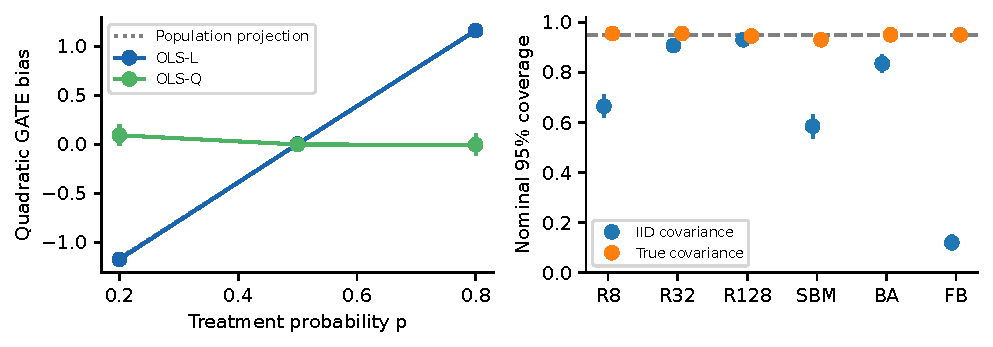
\includegraphics[width=.90\textwidth]{../figures/symmetry_coverage.pdf}
\caption{Left: quadratic-response bias under unequal saturation, degree 32, 400 repetitions per probability. Dotted curve is the population projection calculation. Right: linear-response OLS-L coverage under cluster assignment and correlated noise ($\rho=.5$), 400 repetitions. Intervals use known true covariance or a deliberately incorrect iid covariance. Bars are $\pm1.96$ MCSE; the horizontal line marks nominal coverage.}
\label{fig:extra}
\end{figure}
The following tables include every regression comparator under every primary law and both designs. Parentheses denote one Monte Carlo SE for RMSE; exact bias estimates and other diagnostics are in \texttt{results/main\_summary.csv}. Tables describe the fixed graph realizations. Because several response laws are exactly representable by OLS-C and share identical noise, some empirical RMSEs coincide across laws; these are computed values, not duplicated simulated outcomes.
\begin{table*}[t]
\centering\scriptsize
\caption{Linear response: RMSE (Monte Carlo SE), 400 repetitions.}
\begin{tabular}{llcccccc}
\toprule
Graph & Assignment & DM & OLS-L & OLS-Q & OLS-C & OLS-2H & Ridge-C \\
\midrule
Regular 8 & Bern. & $1.999\,(0.002)$ & $0.076\,(0.003)$ & $0.076\,(0.003)$ & $0.210\,(0.008)$ & $0.208\,(0.007)$ & $0.209\,(0.008)$ \\
Regular 8 & Cluster & $1.385\,(0.002)$ & $0.065\,(0.002)$ & $0.070\,(0.003)$ & $0.137\,(0.005)$ & $0.167\,(0.006)$ & $0.132\,(0.005)$ \\
Regular 32 & Bern. & $2.000\,(0.002)$ & $0.146\,(0.006)$ & $0.150\,(0.006)$ & $1.963\,(0.074)$ & $0.815\,(0.028)$ & $1.912\,(0.072)$ \\
Regular 32 & Cluster & $1.763\,(0.002)$ & $0.142\,(0.006)$ & $0.192\,(0.011)$ & $1.510\,(0.052)$ & $0.729\,(0.026)$ & $1.423\,(0.049)$ \\
Regular 128 & Bern. & $2.001\,(0.002)$ & $0.293\,(0.010)$ & $0.297\,(0.010)$ & $16.519\,(0.641)$ & $3.526\,(0.125)$ & $16.055\,(0.629)$ \\
Regular 128 & Cluster & $1.915\,(0.002)$ & $0.281\,(0.011)$ & $0.510\,(0.034)$ & $15.044\,(0.572)$ & $3.524\,(0.128)$ & $12.454\,(0.467)$ \\
SBM & Bern. & $2.003\,(0.002)$ & $0.136\,(0.005)$ & $0.137\,(0.005)$ & $1.441\,(0.056)$ & $0.220\,(0.009)$ & $1.413\,(0.055)$ \\
SBM & Cluster & $0.300\,(0.002)$ & $0.045\,(0.001)$ & $0.046\,(0.002)$ & $0.057\,(0.002)$ & $0.214\,(0.008)$ & $0.063\,(0.002)$ \\
BA & Bern. & $2.001\,(0.002)$ & $0.130\,(0.004)$ & $0.132\,(0.005)$ & $0.999\,(0.036)$ & $0.767\,(0.027)$ & $0.977\,(0.035)$ \\
BA & Cluster & $1.728\,(0.002)$ & $0.112\,(0.004)$ & $0.143\,(0.007)$ & $0.829\,(0.031)$ & $0.750\,(0.027)$ & $0.783\,(0.028)$ \\
Facebook & Bern. & $2.001\,(0.001)$ & $0.056\,(0.002)$ & $0.059\,(0.002)$ & $0.085\,(0.003)$ & $0.122\,(0.004)$ & $0.084\,(0.003)$ \\
Facebook & Cluster & $0.200\,(0.006)$ & $0.018\,(0.001)$ & $0.019\,(0.001)$ & $0.020\,(0.001)$ & $0.020\,(0.001)$ & $0.021\,(0.001)$ \\
\bottomrule
\end{tabular}
\end{table*}
\begin{table*}[t]
\centering\scriptsize
\caption{Quadratic response: RMSE (Monte Carlo SE), 400 repetitions.}
\begin{tabular}{llcccccc}
\toprule
Graph & Assignment & DM & OLS-L & OLS-Q & OLS-C & OLS-2H & Ridge-C \\
\midrule
Regular 8 & Bern. & $2.000\,(0.002)$ & $0.089\,(0.003)$ & $0.076\,(0.003)$ & $0.210\,(0.008)$ & $0.211\,(0.007)$ & $0.209\,(0.008)$ \\
Regular 8 & Cluster & $1.388\,(0.003)$ & $0.226\,(0.008)$ & $0.070\,(0.003)$ & $0.137\,(0.005)$ & $0.292\,(0.010)$ & $0.132\,(0.005)$ \\
Regular 32 & Bern. & $2.000\,(0.002)$ & $0.151\,(0.006)$ & $0.150\,(0.006)$ & $1.963\,(0.074)$ & $0.813\,(0.029)$ & $1.913\,(0.072)$ \\
Regular 32 & Cluster & $1.764\,(0.002)$ & $0.285\,(0.010)$ & $0.192\,(0.011)$ & $1.510\,(0.052)$ & $0.797\,(0.030)$ & $1.424\,(0.049)$ \\
Regular 128 & Bern. & $2.001\,(0.002)$ & $0.296\,(0.010)$ & $0.297\,(0.010)$ & $16.519\,(0.641)$ & $3.527\,(0.126)$ & $16.056\,(0.629)$ \\
Regular 128 & Cluster & $1.915\,(0.002)$ & $0.354\,(0.013)$ & $0.510\,(0.034)$ & $15.044\,(0.572)$ & $3.531\,(0.129)$ & $12.458\,(0.467)$ \\
SBM & Bern. & $2.003\,(0.002)$ & $0.144\,(0.005)$ & $0.137\,(0.005)$ & $1.441\,(0.056)$ & $0.227\,(0.009)$ & $1.413\,(0.055)$ \\
SBM & Cluster & $0.303\,(0.003)$ & $0.070\,(0.002)$ & $0.046\,(0.002)$ & $0.057\,(0.002)$ & $0.225\,(0.008)$ & $0.063\,(0.002)$ \\
BA & Bern. & $2.001\,(0.002)$ & $0.148\,(0.005)$ & $0.132\,(0.005)$ & $0.999\,(0.036)$ & $0.774\,(0.027)$ & $0.977\,(0.035)$ \\
BA & Cluster & $1.729\,(0.002)$ & $0.280\,(0.010)$ & $0.143\,(0.007)$ & $0.829\,(0.031)$ & $0.819\,(0.029)$ & $0.786\,(0.029)$ \\
Facebook & Bern. & $2.001\,(0.001)$ & $0.172\,(0.006)$ & $0.059\,(0.002)$ & $0.085\,(0.003)$ & $0.151\,(0.005)$ & $0.084\,(0.003)$ \\
Facebook & Cluster & $0.203\,(0.006)$ & $0.041\,(0.002)$ & $0.019\,(0.001)$ & $0.020\,(0.001)$ & $0.045\,(0.002)$ & $0.021\,(0.001)$ \\
\bottomrule
\end{tabular}
\end{table*}
\begin{table*}[t]
\centering\scriptsize
\caption{Cubic response: RMSE (Monte Carlo SE), 400 repetitions.}
\begin{tabular}{llcccccc}
\toprule
Graph & Assignment & DM & OLS-L & OLS-Q & OLS-C & OLS-2H & Ridge-C \\
\midrule
Regular 8 & Bern. & $2.000\,(0.002)$ & $0.351\,(0.005)$ & $0.341\,(0.004)$ & $0.210\,(0.008)$ & $0.398\,(0.010)$ & $0.207\,(0.008)$ \\
Regular 8 & Cluster & $1.483\,(0.005)$ & $0.423\,(0.013)$ & $0.289\,(0.004)$ & $0.137\,(0.005)$ & $0.473\,(0.015)$ & $0.132\,(0.005)$ \\
Regular 32 & Bern. & $2.000\,(0.002)$ & $0.477\,(0.007)$ & $0.478\,(0.007)$ & $1.963\,(0.074)$ & $0.942\,(0.031)$ & $1.911\,(0.072)$ \\
Regular 32 & Cluster & $1.816\,(0.003)$ & $0.582\,(0.016)$ & $0.495\,(0.009)$ & $1.510\,(0.052)$ & $0.966\,(0.034)$ & $1.425\,(0.049)$ \\
Regular 128 & Bern. & $2.001\,(0.002)$ & $0.577\,(0.013)$ & $0.582\,(0.013)$ & $16.519\,(0.641)$ & $3.610\,(0.128)$ & $16.046\,(0.628)$ \\
Regular 128 & Cluster & $1.934\,(0.002)$ & $0.624\,(0.019)$ & $0.718\,(0.027)$ & $15.044\,(0.572)$ & $3.537\,(0.130)$ & $12.443\,(0.466)$ \\
SBM & Bern. & $2.003\,(0.002)$ & $0.467\,(0.007)$ & $0.467\,(0.007)$ & $1.441\,(0.056)$ & $0.511\,(0.011)$ & $1.408\,(0.055)$ \\
SBM & Cluster & $0.410\,(0.004)$ & $0.095\,(0.003)$ & $0.054\,(0.002)$ & $0.057\,(0.002)$ & $0.240\,(0.008)$ & $0.051\,(0.002)$ \\
BA & Bern. & $2.001\,(0.002)$ & $0.471\,(0.008)$ & $0.459\,(0.006)$ & $0.999\,(0.036)$ & $0.902\,(0.031)$ & $0.976\,(0.035)$ \\
BA & Cluster & $1.785\,(0.003)$ & $0.564\,(0.015)$ & $0.466\,(0.008)$ & $0.829\,(0.031)$ & $0.995\,(0.032)$ & $0.788\,(0.029)$ \\
Facebook & Bern. & $2.001\,(0.001)$ & $0.333\,(0.010)$ & $0.235\,(0.003)$ & $0.085\,(0.003)$ & $0.412\,(0.009)$ & $0.085\,(0.003)$ \\
Facebook & Cluster & $0.230\,(0.007)$ & $0.059\,(0.002)$ & $0.028\,(0.001)$ & $0.020\,(0.001)$ & $0.064\,(0.002)$ & $0.020\,(0.001)$ \\
\bottomrule
\end{tabular}
\end{table*}
\begin{table*}[t]
\centering\scriptsize
\caption{Threshold response: RMSE (Monte Carlo SE), 400 repetitions.}
\begin{tabular}{llcccccc}
\toprule
Graph & Assignment & DM & OLS-L & OLS-Q & OLS-C & OLS-2H & Ridge-C \\
\midrule
Regular 8 & Bern. & $2.000\,(0.002)$ & $1.148\,(0.008)$ & $1.146\,(0.005)$ & $1.597\,(0.019)$ & $1.167\,(0.014)$ & $1.532\,(0.019)$ \\
Regular 8 & Cluster & $1.681\,(0.008)$ & $0.846\,(0.021)$ & $0.719\,(0.008)$ & $1.065\,(0.013)$ & $0.905\,(0.024)$ & $1.016\,(0.013)$ \\
Regular 32 & Bern. & $1.999\,(0.002)$ & $1.982\,(0.007)$ & $1.988\,(0.008)$ & $2.783\,(0.087)$ & $2.162\,(0.039)$ & $2.735\,(0.085)$ \\
Regular 32 & Cluster & $1.986\,(0.002)$ & $1.849\,(0.014)$ & $2.208\,(0.049)$ & $5.527\,(0.366)$ & $2.015\,(0.039)$ & $4.719\,(0.260)$ \\
Regular 128 & Bern. & $2.000\,(0.002)$ & $2.026\,(0.014)$ & $2.033\,(0.015)$ & $16.642\,(0.629)$ & $4.225\,(0.142)$ & $16.159\,(0.610)$ \\
Regular 128 & Cluster & $1.998\,(0.002)$ & $2.025\,(0.014)$ & $2.070\,(0.024)$ & $15.316\,(0.588)$ & $3.928\,(0.138)$ & $12.632\,(0.463)$ \\
SBM & Bern. & $2.002\,(0.002)$ & $1.944\,(0.008)$ & $1.958\,(0.007)$ & $2.291\,(0.077)$ & $1.970\,(0.012)$ & $2.234\,(0.075)$ \\
SBM & Cluster & $0.053\,(0.002)$ & $0.107\,(0.003)$ & $0.133\,(0.006)$ & $0.117\,(0.003)$ & $0.234\,(0.008)$ & $0.133\,(0.005)$ \\
BA & Bern. & $2.000\,(0.002)$ & $1.830\,(0.009)$ & $1.854\,(0.008)$ & $2.542\,(0.081)$ & $1.992\,(0.039)$ & $2.460\,(0.079)$ \\
BA & Cluster & $1.957\,(0.003)$ & $1.599\,(0.020)$ & $1.982\,(0.035)$ & $4.367\,(0.162)$ & $1.882\,(0.041)$ & $4.092\,(0.146)$ \\
Facebook & Bern. & $2.001\,(0.001)$ & $0.834\,(0.017)$ & $0.809\,(0.007)$ & $0.164\,(0.004)$ & $1.371\,(0.013)$ & $0.156\,(0.004)$ \\
Facebook & Cluster & $0.188\,(0.006)$ & $0.067\,(0.002)$ & $0.066\,(0.002)$ & $0.043\,(0.002)$ & $0.068\,(0.002)$ & $0.057\,(0.002)$ \\
\bottomrule
\end{tabular}
\end{table*}
\begin{table*}[t]
\centering\scriptsize
\caption{Twohop response: RMSE (Monte Carlo SE), 400 repetitions.}
\begin{tabular}{llcccccc}
\toprule
Graph & Assignment & DM & OLS-L & OLS-Q & OLS-C & OLS-2H & Ridge-C \\
\midrule
Regular 8 & Bern. & $1.874\,(0.002)$ & $0.883\,(0.004)$ & $0.882\,(0.004)$ & $0.896\,(0.010)$ & $0.208\,(0.007)$ & $0.886\,(0.010)$ \\
Regular 8 & Cluster & $1.500\,(0.002)$ & $0.627\,(0.003)$ & $0.627\,(0.004)$ & $0.647\,(0.007)$ & $0.167\,(0.006)$ & $0.633\,(0.007)$ \\
Regular 32 & Bern. & $1.969\,(0.002)$ & $0.979\,(0.007)$ & $0.979\,(0.007)$ & $2.234\,(0.077)$ & $0.815\,(0.028)$ & $2.148\,(0.074)$ \\
Regular 32 & Cluster & $1.840\,(0.002)$ & $0.865\,(0.007)$ & $0.878\,(0.009)$ & $1.769\,(0.060)$ & $0.729\,(0.026)$ & $1.680\,(0.056)$ \\
Regular 128 & Bern. & $1.993\,(0.002)$ & $1.041\,(0.014)$ & $1.048\,(0.014)$ & $16.548\,(0.636)$ & $3.526\,(0.125)$ & $16.044\,(0.619)$ \\
Regular 128 & Cluster & $1.948\,(0.002)$ & $0.998\,(0.014)$ & $1.086\,(0.025)$ & $15.139\,(0.578)$ & $3.524\,(0.128)$ & $12.493\,(0.463)$ \\
SBM & Bern. & $1.967\,(0.002)$ & $0.580\,(0.007)$ & $0.584\,(0.007)$ & $1.661\,(0.065)$ & $0.220\,(0.009)$ & $1.578\,(0.062)$ \\
SBM & Cluster & $0.419\,(0.002)$ & $0.154\,(0.002)$ & $0.154\,(0.002)$ & $0.158\,(0.003)$ & $0.214\,(0.008)$ & $0.115\,(0.002)$ \\
BA & Bern. & $1.970\,(0.002)$ & $0.986\,(0.007)$ & $0.986\,(0.007)$ & $1.421\,(0.044)$ & $0.767\,(0.027)$ & $1.374\,(0.043)$ \\
BA & Cluster & $1.821\,(0.002)$ & $0.880\,(0.006)$ & $0.884\,(0.007)$ & $1.235\,(0.036)$ & $0.750\,(0.027)$ & $1.191\,(0.034)$ \\
Facebook & Bern. & $1.961\,(0.001)$ & $0.757\,(0.003)$ & $0.749\,(0.003)$ & $0.891\,(0.005)$ & $0.122\,(0.004)$ & $0.891\,(0.005)$ \\
Facebook & Cluster & $0.244\,(0.006)$ & $0.057\,(0.001)$ & $0.057\,(0.001)$ & $0.053\,(0.001)$ & $0.020\,(0.001)$ & $0.047\,(0.001)$ \\
\bottomrule
\end{tabular}
\end{table*}
\clearpage
\section{Threshold Oracle: Estimability Is an Outcome}\label{app:oracle}
The oracle uses the correct feature dictionary $(1,x,z,\one(s\ge.8))$, with endpoint contrast $(0,0,1,1)$. If its indicator column is absent or its contrast is otherwise outside the observed row space, the run is marked inestimable. Conditional-on-estimability error is not the unconditional error of a deployable estimator; no fallback is silently supplied. Threshold oracle results are regenerated using the main assignments and noise, and are stored separately.
\begin{table}[h]\centering\small
\caption{Correct threshold regression: estimability counts and RMSE conditional on estimability. A dash means no contrast was estimable.}
\begin{tabular}{llrrr}
\toprule
Graph & Design & Estimable/400 & RMSE if estimable & MCSE \\
\midrule
Regular 8 & bernoulli & 400 & 0.081 & 0.003 \\
Regular 8 & cluster & 400 & 0.054 & 0.002 \\
Regular 32 & bernoulli & 127 & 0.478 & 0.036 \\
Regular 32 & cluster & 247 & 0.330 & 0.023 \\
Regular 128 & bernoulli & 0 & --- & --- \\
Regular 128 & cluster & 0 & --- & --- \\
SBM & bernoulli & 266 & 0.416 & 0.020 \\
SBM & cluster & 400 & 0.024 & 0.001 \\
BA & bernoulli & 391 & 0.291 & 0.015 \\
BA & cluster & 371 & 0.233 & 0.014 \\
Facebook & bernoulli & 400 & 0.052 & 0.002 \\
Facebook & cluster & 400 & 0.017 & 0.001 \\
\bottomrule
\end{tabular}
\end{table}

\section{Full-Exposure HT and Rare Events}\label{app:ht}
All four one-hop response laws have identical outcomes under closed-neighborhood full treatment/control exposure, and thus exactly the same realized HT estimates when sharing noise. The two-hop response does not share this exposure mapping: neighbors' neighbors remain relevant, so the displayed HT would be misspecified for that law. Its invalidity is recorded rather than interpreted as a valid unbiased comparison.

Even for one-hop laws, inverse exposure probabilities may be astronomically large. If no full exposures occur in a repetition, HT returns zero, not a missing estimate. This makes the repeated-simulation distribution look misleadingly concentrated around an incorrect value before extremely rare events are observed. The table reports that behavior explicitly. Empirical Monte Carlo SEs can be zero when all repetitions miss the tail; they must not be read as evidence that the true estimator variance or MSE is small. We did not attempt importance sampling or an exact joint-exposure variance calculation on the large graphs. The theoretical one-hop unbiasedness does not conflict with the highly nonzero empirical mean errors at this repetition budget.
\begin{table}[h]\centering\small
\caption{One-hop cubic-response HT: observed finite-budget behavior, not a resolved estimate of its rare-tail risk. RMSE MCSE is the empirical delta-method value and can severely understate uncertainty.}
\begin{tabular}{llrrrr}
\toprule
Graph & Design & No exposures/400 & Mean estimate & Empirical RMSE & MCSE \\
\midrule
Regular 8 & bernoulli & 2 & 2.712 & 2.399 & 0.090 \\
Regular 8 & cluster & 0 & 2.785 & 4.484 & 0.249 \\
Regular 32 & bernoulli & 400 & 0.000 & 3.000 & 0.000 \\
Regular 32 & cluster & 400 & 0.000 & 3.000 & 0.000 \\
Regular 128 & bernoulli & 400 & 0.000 & 3.000 & 0.000 \\
Regular 128 & cluster & 400 & 0.000 & 3.000 & 0.000 \\
SBM & bernoulli & 399 & 2.576 & 51.452 & 25.639 \\
SBM & cluster & 0 & 2.922 & 3.990 & 0.193 \\
BA & bernoulli & 400 & 0.000 & 3.000 & 0.000 \\
BA & cluster & 360 & 2.972 & 31.382 & 10.357 \\
Facebook & bernoulli & 0 & 2.156 & 22.431 & 10.826 \\
Facebook & cluster & 0 & 2.836 & 3.021 & 0.132 \\
\bottomrule
\end{tabular}
\end{table}

\section{Sensitivity Coverage and Interval Width}
Table~\ref{tab:senscoverage} reports the precision cost of the curvature guarantee for the cubic law using $M=12$ and the true iid noise variance. Sensitivity intervals use \eqref{eq:ci}; Gaussian-only intervals omit the bias bound. Wilson intervals quantify finite-repetition uncertainty in coverage, including all-success cases where an empirical binomial standard error would be zero. The guarantee is conditional and worst-case over the smooth response class; high empirical coverage for this one law does not establish a smaller valid curvature constant. These trials regenerate primary assignments and are not independent additional data.
\begin{table}[h]\centering\scriptsize
\caption{OLS-L, cubic law, 400 repetitions per graph/design: coverage and average sensitivity half-width (in GATE units). Coverage uncertainty is a 95\% Wilson interval; width uncertainty is one Monte Carlo SE. Covariance and $M$ are supplied, not estimated.}\label{tab:senscoverage}
\begin{tabular}{llrrrr}
\toprule
Graph & Design & Gaussian coverage & Sensitivity coverage [95\% Wilson CI] & Half-width & MCSE \\
\midrule
BA & bernoulli & 14.5\% & 100.00\% [99.05, 100.00] & 2.244 & 0.002 \\
BA & cluster & 24.5\% & 100.00\% [99.05, 100.00] & 2.162 & 0.006 \\
Facebook & bernoulli & 22.5\% & 100.00\% [99.05, 100.00] & 1.104 & 0.005 \\
Facebook & cluster & 45.8\% & 100.00\% [99.05, 100.00] & 0.135 & 0.003 \\
SBM & bernoulli & 13.5\% & 100.00\% [99.05, 100.00] & 2.362 & 0.003 \\
SBM & cluster & 65.2\% & 99.75\% [98.60, 99.96] & 0.247 & 0.004 \\
Regular 128 & bernoulli & 60.8\% & 100.00\% [99.05, 100.00] & 3.177 & 0.001 \\
Regular 128 & cluster & 62.0\% & 100.00\% [99.05, 100.00] & 3.177 & 0.003 \\
Regular 32 & bernoulli & 13.0\% & 100.00\% [99.05, 100.00] & 2.455 & 0.001 \\
Regular 32 & cluster & 28.2\% & 100.00\% [99.05, 100.00] & 2.376 & 0.005 \\
Regular 8 & bernoulli & 4.0\% & 100.00\% [99.05, 100.00] & 1.517 & 0.002 \\
Regular 8 & cluster & 19.8\% & 100.00\% [99.05, 100.00] & 1.273 & 0.008 \\
\bottomrule
\end{tabular}
\end{table}

\clearpage
\section{Reproducibility and Responsible Research Record}
The package contains the complete simulation code, pinned Python environment, raw per-repetition results, generated tables/figures, official ICML 2026 style files, LaTeX source, compiled PDF, and a command-by-command reproduction guide. No GPU or paid service is required. Only the public SNAP edge list is downloaded; its SHA-256 is verified by the acquisition script and recorded in the manifest. The dataset page gives a citation but no explicit redistribution license; the reproducible archive therefore supplies acquisition code, while a local downloaded copy is retained in the working directory. No proprietary experimental data are used.

The initial design was recorded in \texttt{EXPERIMENT\_PLAN.md} before the main simulations. The Peano-kernel refinement and threshold oracle were added after implementing the initial decomposition; the support ablation was an exploratory response to public-graph results. All evaluated fixed models, including unsuccessful ridge, RF, and unsupported threshold fits, are reported. No adaptive graph-feature selection, GNN, rollout experiment, or feasible covariance estimator was implemented or presented as completed. A failed direct source-paper download is recorded in the access log; that paper was not cited as a consulted source. Literature access was restricted to the provided starter papers, the public graph page, and official conference-format pages. No prohibited-work encounter was observed during this restricted access. The source access log records the consulted sections and exact URLs.

This study was designed, implemented, analyzed, and written by an autonomous language-model coding agent at the user's request. No human-subject experiment occurred, no real treatment effects were estimated, and no external human author or affiliation is claimed. All reported empirical numbers are produced by the included code from actual runs. The anonymous conference format is used to satisfy the requested paper style, not to claim submission, acceptance, or human authorship.

\subsection*{Completed reproducibility checklist}
ICML 2026's downloaded official template and author instructions do not include a separate NeurIPS-style paper checklist. Its required impact statement appears above. We additionally complete the following explicit checklist for this artifact; this is our reporting checklist, not an invented official ICML form.
\begin{enumerate}[leftmargin=*,itemsep=1pt]
\item \textbf{Claims match evidence: Yes.} The main text distinguishes exact identities/theorems from finite-graph simulation and population-Gram proxies. No universal ranking or topology-wide rate is claimed.
\item \textbf{Assumptions and proofs: Yes.} Curvature, homogeneity, calibration, estimability, exogeneity, and known covariance are stated; proofs appear in Appendix~\ref{app:proofs}. Unsupported response laws are excluded from sensitivity guarantees.
\item \textbf{Algorithms and experimental details: Yes.} Scripts specify features, seeds, estimability tolerance, penalties, splits, graph construction, groups, and noise. The README lists exact commands and artifact mapping.
\item \textbf{Repetition uncertainty: Yes.} Bias/RMSE MCSE, coverage uncertainty, and paired method-loss comparisons are provided. Graph-realization uncertainty is not estimated. HT's rare tails are explicitly unresolved.
\item \textbf{Code and environment: Yes.} All generation/analysis scripts and fully pinned dependencies are included. CPU execution and build instructions reproduce the paper figures and tables.
\item \textbf{Data provenance: Yes.} Public graph URL, checksum, node/edge verification, preprocessing, access date, citation, and license uncertainty are recorded. All outcomes and assignments are synthetic.
\item \textbf{Failures and exploratory analysis: Yes.} Inestimable threshold fits, poor RF/ridge results, HT tail limitations, the exploratory support ablation and equal-size deletion control, and the failed source download are documented.
\item \textbf{Compute reporting: Yes.} Run JSON files record actual elapsed simulation times on this machine. Reproduction runtimes are identified as machine-dependent; the README records hardware and software.
\item \textbf{Limitations and impact: Yes.} Fixed graph scope, synthetic/homogeneous response, unknown curvature/covariance, partial literature access, and public-data ethics are discussed.
\item \textbf{Human participants or private data: Not applicable.} No participants were recruited and no private experimental data or node attributes were used.
\item \textbf{External access restrictions: Yes.} No broad literature search was performed. Only approved starting papers and necessary official/data pages were accessed; the access log reports what was read.
\end{enumerate}
\end{document}
